\documentclass{article}
\usepackage{graphicx}
\usepackage{float}
\usepackage[spanish]{babel}
\usepackage{hyperref}
\usepackage{csquotes}
\graphicspath{ {img/} }
\setlength{\parskip}{\baselineskip}

\title{Persistencia de Datos \\[3ex] \small PAMN - Programación de Aplicaciónes Moviles Nativas}

\author{Chamil José Cruz Razeq}

\begin{document}
    \maketitle
    \thispagestyle{empty}
    \newpage

    \section{Introducción}
        Todas las tareas propuestas se encuentran disponibles en el siguiente
         repositorio de \href{https://github.com/chamilstudy/ulpgc_pamn_assigments}{GitHub},
         siendo esta la correspondiente a la entrega 8.

    \section{Codelabs 1. Persistencia de datos con Room}
        Para este primer ejercicio se plantéa un sencillo programa que permite la creación
         de listas de objetos definidos por:
         \begin{itemize}
            \item Nombre
            \item Valor
            \item Cantidad
         \end{itemize}
        Con la posibilidad de editar sus características y incrementar/decrementar su
        cantidad.

        La interfaz viene facilitada en un repositorio \href{https://github.com/google-developer-training/basic-android-kotlin-compose-training-inventory-app.git}{github}.
        A lo largo de la resolución se plantea la implementación mediante Rooms de:

        \begin{itemize}
            \item Persistencia de Datos
            Se trabaja sobre el modelo y la vista-modelo, implementando:
            \begin{itemize}
                \item Entity, que definirá los atributos (o datos).
                \item DAO, que definirá la interfaz de las funciones que servirán de
                        gestión sobre la base de datos, estableciendo "QUERIES" y "FLUJOS".
                \item Instancia, función que retornará la instancia de la base de datos.
                \item Repositorio, que servirá como implementación de la interfaz DAO.
            \end{itemize}
            Finalmente se ha implementado la función guardar que permite, a través del formulario [ Figura \ref{fig:codelab2_2} ],
             guardar en la BBDD un item con los valores definidos. No obstante, no será hasta la resolución
             del siguiente punto que estos se muestren en la lista de items, y pueda interactuarse con ellos.
            \item Lectura y Escritura
            Se trabaja sobre la vista-modelo y la vista, implementando:
            \begin{itemize}
                \item Actualización de los elementos visuales de la aplicación para que muestren los
                       items [ Figura \ref{fig:codelab2_3} ], se pueda interactuar con ellos [ Figura \ref{fig:codelab2_2} ]
                       y puedan ser editados, estableciendo en los campos del formulario los valores del item
                       seleccionado [ Figura \ref{fig:codelab2_1} ].
                \item Pruebas sobre la BBDD, creando ficheros para realizar consultas de prueba y verificar que
                       lo implementado en el modelo y vista-modelo funciona adecuadamente.
            \end{itemize}
        \end{itemize}

        \begin{figure}[H]
            \centerline{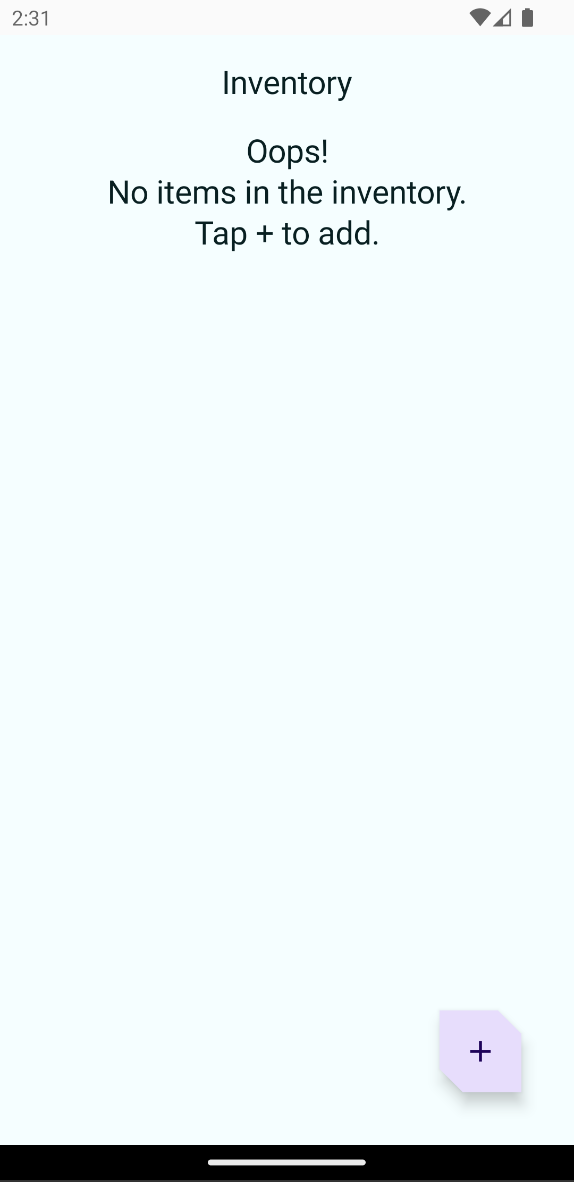
\includegraphics[scale=0.3]{codelab2_1.png}}
            \caption{Lista de items vacía}
            \label{fig:codelab2_1}
        \end{figure}
        \begin{figure}[H]
            \centerline{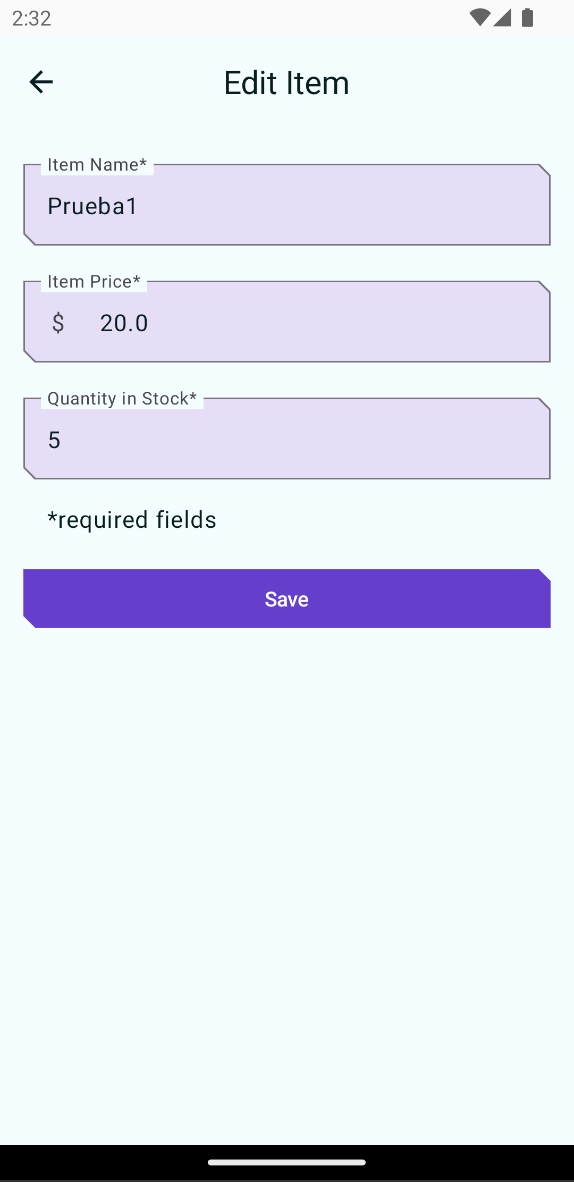
\includegraphics[scale=0.3]{codelab2_2.png}}
            \caption{Formulario de creación/edición de items}
            \label{fig:codelab2_2}
        \end{figure}
        \begin{figure}[H]
            \centerline{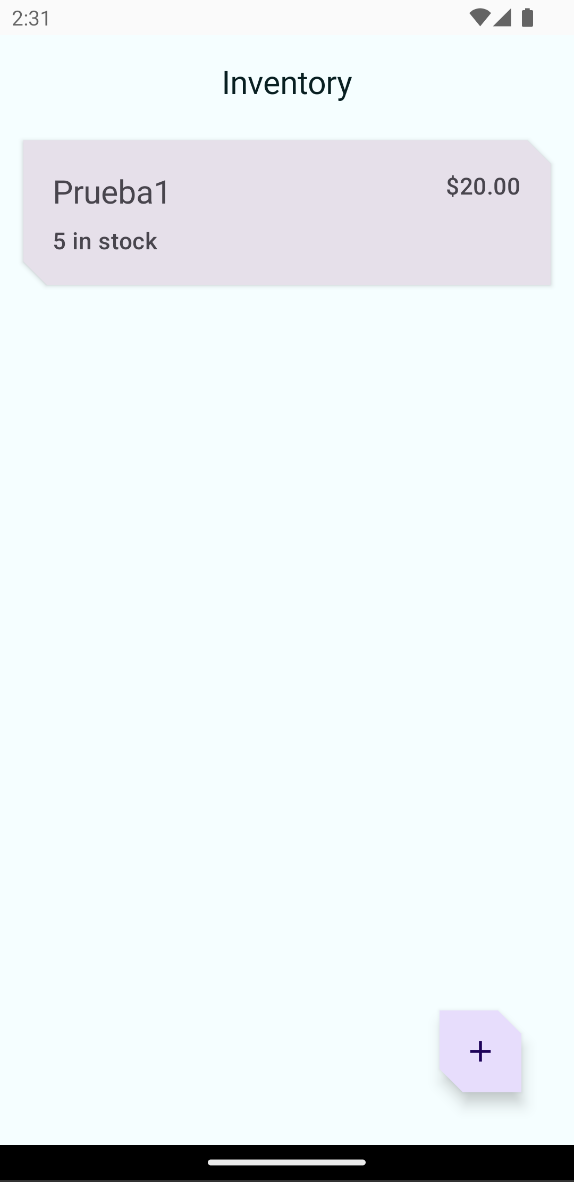
\includegraphics[scale=0.3]{codelab2_3.png}}
            \caption{Lista de items con un item}
            \label{fig:codelab2_3}
        \end{figure}
        \begin{figure}[H]
            \centerline{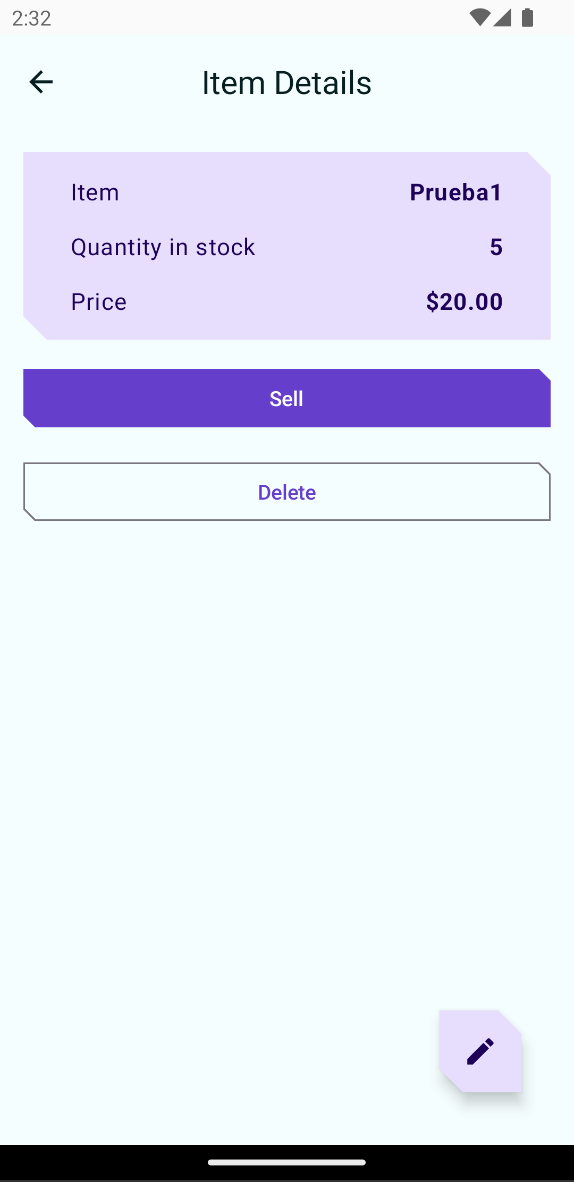
\includegraphics[scale=0.3]{codelab2_4.png}}
            \caption{Interacción con item}
            \label{fig:codelab2_4}
        \end{figure}

    \section{Codelabs 2. Persistencia de ajustes de usuario}
        En este segundo ejercicio se plantea un sencillo programa donde se ofrece al usuario
         la posibilidad de establecer una vista en lista [ Figura \ref{fig:codelab2.1_1} ] o
         en cuadrícula [ Figura \ref{fig:codelab2.1_1} ]. El objetivo es que la elección del
         usuario permanezca tras cerrar la aplicación. Para ello el curso propone hacer uso
         de la dependencia "datastore-preference", donde se implementó:

        \begin{itemize}
            \item El repositorio de preferencias de usuario, donde se han definido
                   los estados de lista y cuadrícula, además del control de excepciones.
            \item La inicialización del DataStore para que garantizar la aplicación
                   de los cambios realizados.
            \item El uso de la información contenida de forma que los elementos visuales
                   se muestren en consecuencia.
        \end{itemize}

        \begin{figure}[H]
            \centerline{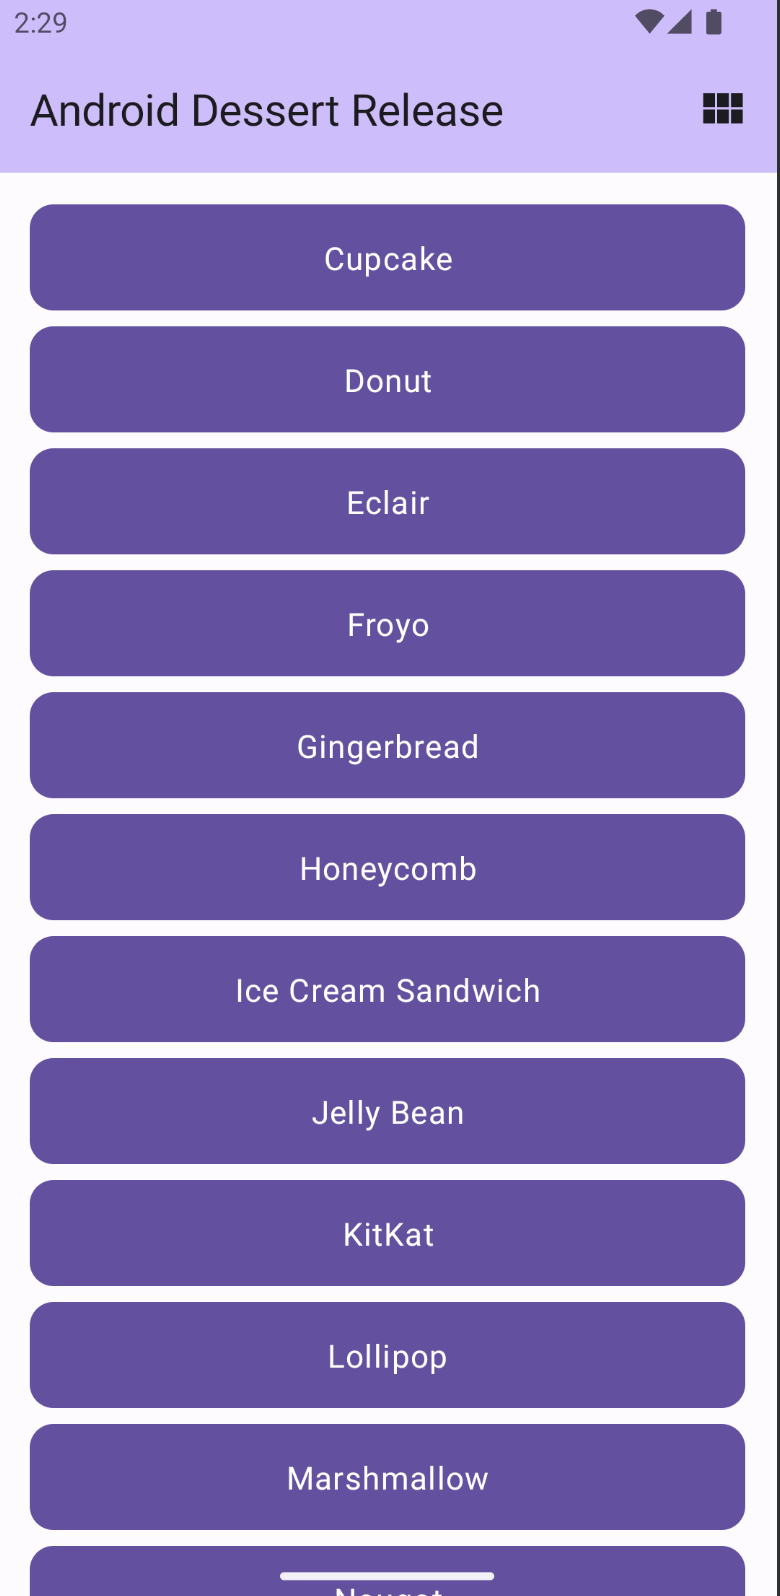
\includegraphics[scale=0.3]{codelab2.1_1.png}}
            \caption{Vista en lista}
            \label{fig:codelab2.1_1}
        \end{figure}
        \begin{figure}[H]
            \centerline{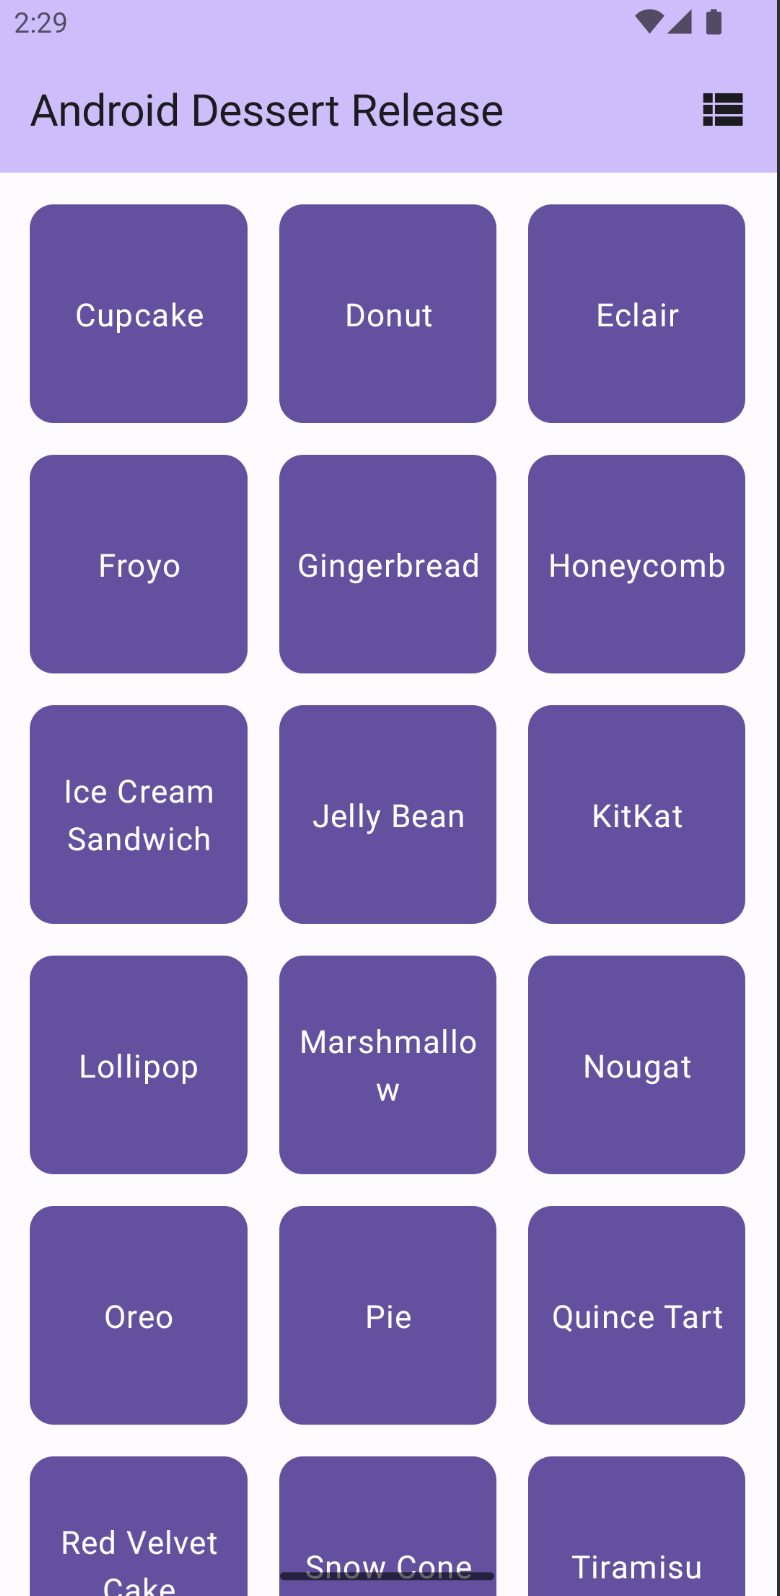
\includegraphics[scale=0.3]{codelab2.1_2.png}}
            \caption{Vista en cuadricula}
            \label{fig:codelab2.1_2}
        \end{figure}

    \section{Conclusión}
    Los ejercicios anteriores fueron completamente guiados, muestran adecuadamente la 
     implementación de las tecnologías propuestas: ROOMS y DATASTORE, además de poner
     en práctica la arquitectura MVVM, no obstante se planteán ejercicios adicionales
     para poner en práctica dificiles de implementar por problemas a la hora de agregar
     las dependencias, que fallan por diversos motivos (versionado o código obsoleto),
     provocando que para poder finalizarlos haya que hacer cierto sobresfuerzo.
     Considero que este apartado tan crucial del desarrollo debería abordarse de otra
     forma ya que los cursos ofrecidos por "Google" no cumplen con todas las garantías.

    \begin{thebibliography}{}
        \bibitem{lab3} PAMN Lab3 Arquitectura
        \bibitem{RoomsVSSQLite} Rooms - https://medium.com/dvt-engineering/android-room-versus-sqlite-which-is-best-32ff651bc361
    \end{thebibliography}
        
\end{document}
